\chapter{The LHCb detector}
\label{chap:dec}
In this section, overview of accelator complex at CERN as well as physics motivation behind \Gls{LHCb} detector and its details will be described.

CERN built one of the most exciting laboratories to study elementary particle interactions. The complex set of particle accelerators and detectors is shown in \autoref{fig:AcceleratorComplex}. The proccess of accelerating protons starts with the source of protons. Protons are obtained from hydrogen gas bottle by applying and an electric field seperates hydrogen into positively and negatively charged constituents. The first proton accelerator in the chain, Linac 2, accelerates the protons to the energy of 50 MeV. Is is a tank composed of several chambers where the resonant cavity is tuned to a specific frequency which creates potential differences in the cavities making accelerate the protons. These are then injected into the Proton Synchrotron Booster (PSB). Here the protons are accelerated to 1.4 GeV. The next line is the Proton Synchrotron (PS) reaching energy of 25 GeV. Before either entering the LHC or North Area (mainly used as testing facility for experiment upgrades) Super Proton Synchrotron (SPS) is the last stop. Here proton acceleration to 450 GeV is achieved.

\begin{figure}
  \centering
  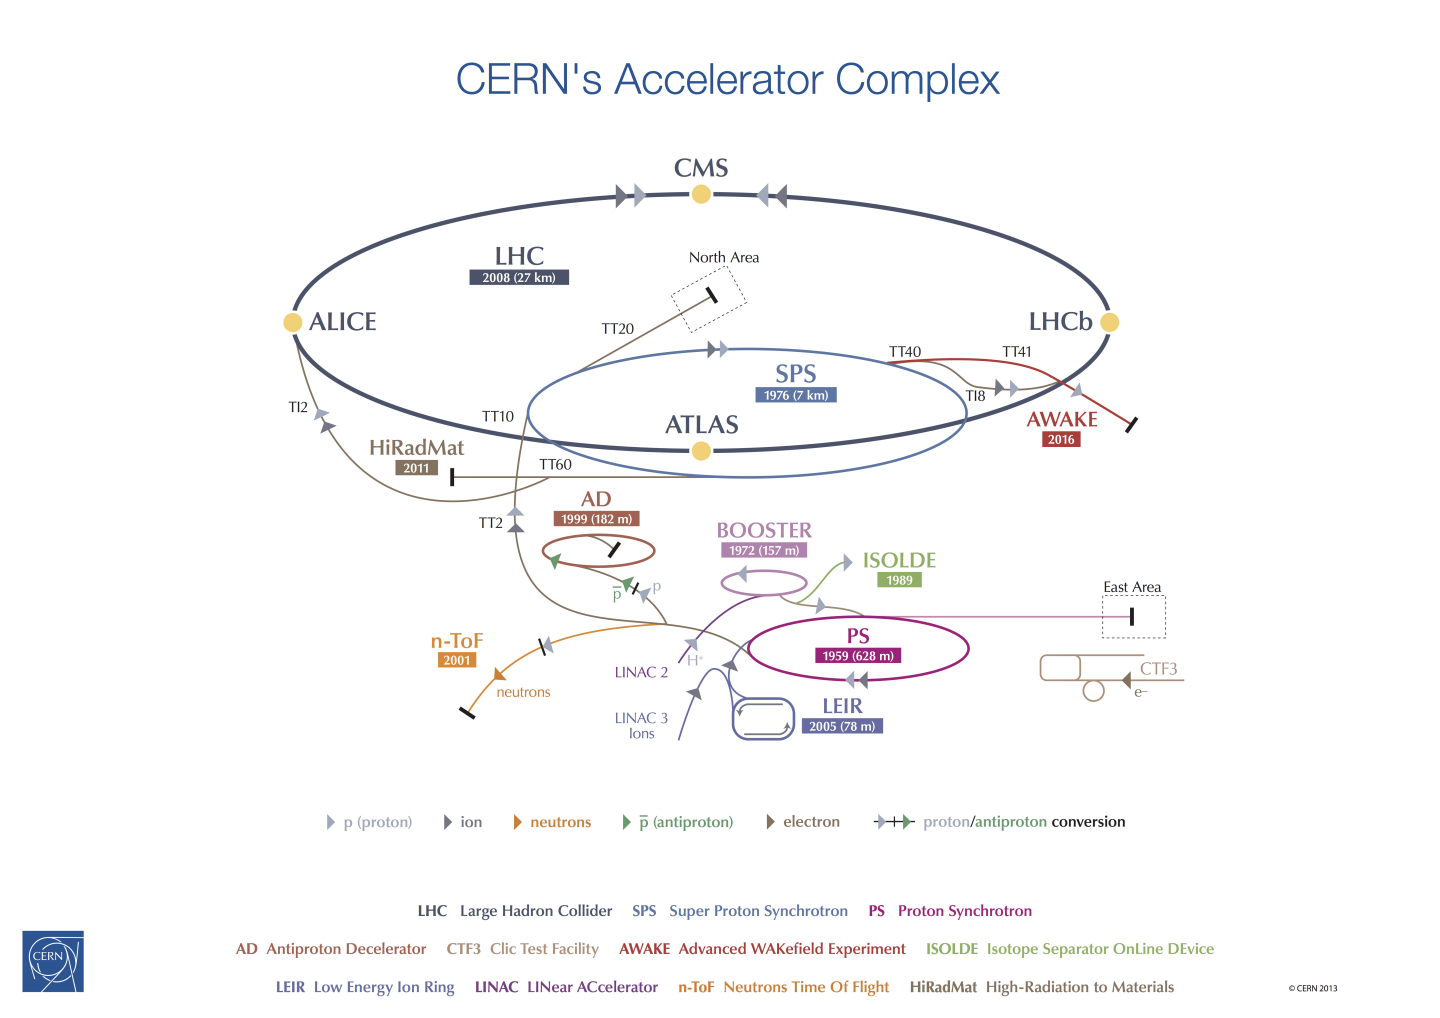
\includegraphics[scale = 0.5]{figs/detector/AccComplex.jpg}
  \caption{Accelerator complex at CERN}
  \label{fig:AcceleratorComplex}
\end{figure}

The Large Hadron Collider (LHC) is a complex machine which accelerates beams of protons in opposite directions in $\sim$ 27km circular tunnel. It is located
50-157\m below ground on the border of Switzerland and France. Once the desired energy is achieved proton-proton, $pp$, or ion, collisions happen at four distinct points, where different detectors with different physics focus are located. These are \Gls{ATLAS}, \Gls{CMS}, \Gls{ALICE} and \Gls{LHCb}. 
Study of \Bmumumu was performed using data obtained at \Gls{LHCb}. 

\section{LHCb Layout}

\Gls{LHCb} differs from the other general purpose detectors on the LHC ring as its studies properties of heavy particles containing $b$ or $c$ quarks. This can be attributed to the geometrical acceptance and unique vertex resolution as well as excelent \Gls{PID}.

Contrary to the two general purpose detectors where the collisions are occuring in the centre of the detector, \Gls{LHCb}'s collision point is located at one end of the detector, hence its description as a forward single-arm spectrometer. This means that information about products outside of its scope are not known, meaning that there is no overall constraint on collision information, unlike in other flavour experiments. This is compensated by production mechanism of $b\bar{b}$ and $c\bar{c}$ in $pp$ interactions, which occurs via gluon-gluon fusion. In this process, each gluon will carry part of proton's momentum. If the two gluons from two protons carry significantly different momentum, the $b\bar{b}$ system will be boosted with respect to the $pp$ rest frame, either in forward or backward cone closely to the beamline, as can be seen in \autoref{fig:Acceptance}.


\begin{figure}
	\centering
	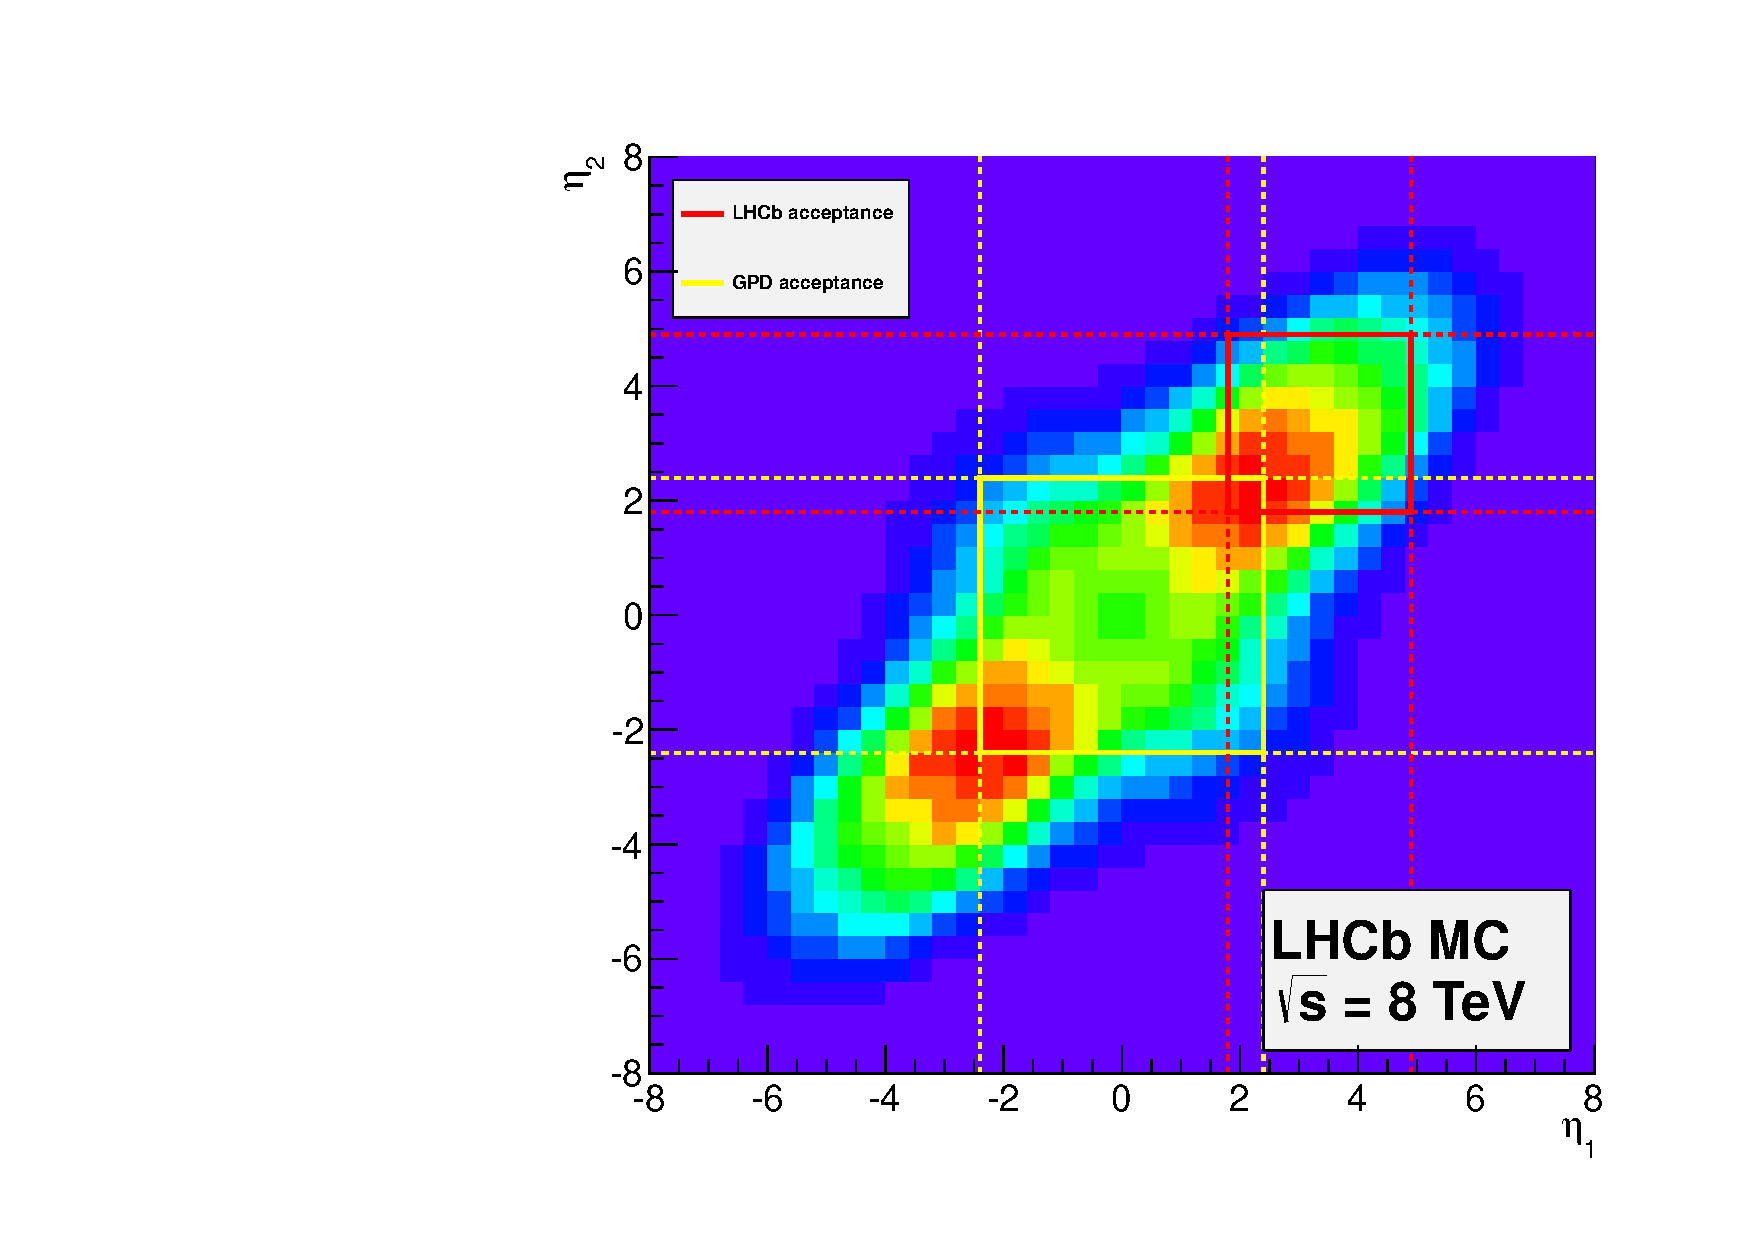
\includegraphics[scale = 0.3]{figs/detector/Acceptance.pdf}
	\caption{Angular production and acceptance of LHCb's $b\bar{b}$ pair (in red) as well as General Purpose Detector (in yellow). LHCb covers region with highest production cross-section at 8 \tev. These plots were produced using PYTHIA8 \cite{pythia8} simulation.}
	\label{fig:Acceptance}
\end{figure}

The angular coverage of LHCb is formally defined using pseudorapidity $\eta$, 

\begin{equation}
	\eta = -\ln (\tan\frac{\theta}{2})
\end{equation}	
where $\theta$ is defined in \autoref{fig:LHCbDetector}. \Gls{LHCb}, hence, covers the region $2<\eta<5$ or 300\mrad. The production cross-section of the fundamental process $pp\rightarrow b\bar{b}X$, $\sigma (pp\rightarrow b\bar{b}X)$= 75.3$\pm$5.4$\pm$13.0 $\upmu$b at 7 \tev \cite{LHCb-PAPER-2010-002} and 144$\pm$1$\pm$21 $\upmu$b at 13 \tev \cite{LHCb-PAPER-2016-031} has been measured.

To limit the background coming from especially soft QCD processes (due to hadronic collision enviroment) global event cuts, \textit{GEC}s, are put in the place. To limit the occupancy of the detector only events with 600 (in 7,8 \tev) and 450 (in 13 \tev) tracks and less are allowed to be processed. In order to achieve these occupancies, $\mu_{vis}$, the average number of visible $pp$ interactions per bunch-crossing is kept below 1, so that the pile-up, the visible number of $pp$ interaction in the visible events, is limited. This LHCb-specific control of luminosity is achieved by \textit{luminosity levelling}. This is procedure that is achieved by controlling the transverse
overlap of the beams at collision point. It allows the instantaneous luminosity to be of the desired value limiting the effects of luminosity decay, which leads to trigger changes while data taking.

So far, the detector has been running since 2010, with diferrent running conditions summarized in Table , and with collected integrated luminosity \autoref{fig:lhcbintlumi}
%Formally LHCb detector is placed along the beamline, where $x,y,z$ a spectrometer which cover the region of 300 \mrad defined a
%http://lhcb.web.cern.ch/lhcb/speakersbureau/excel/default.html


\begin{figure}
	\centering
	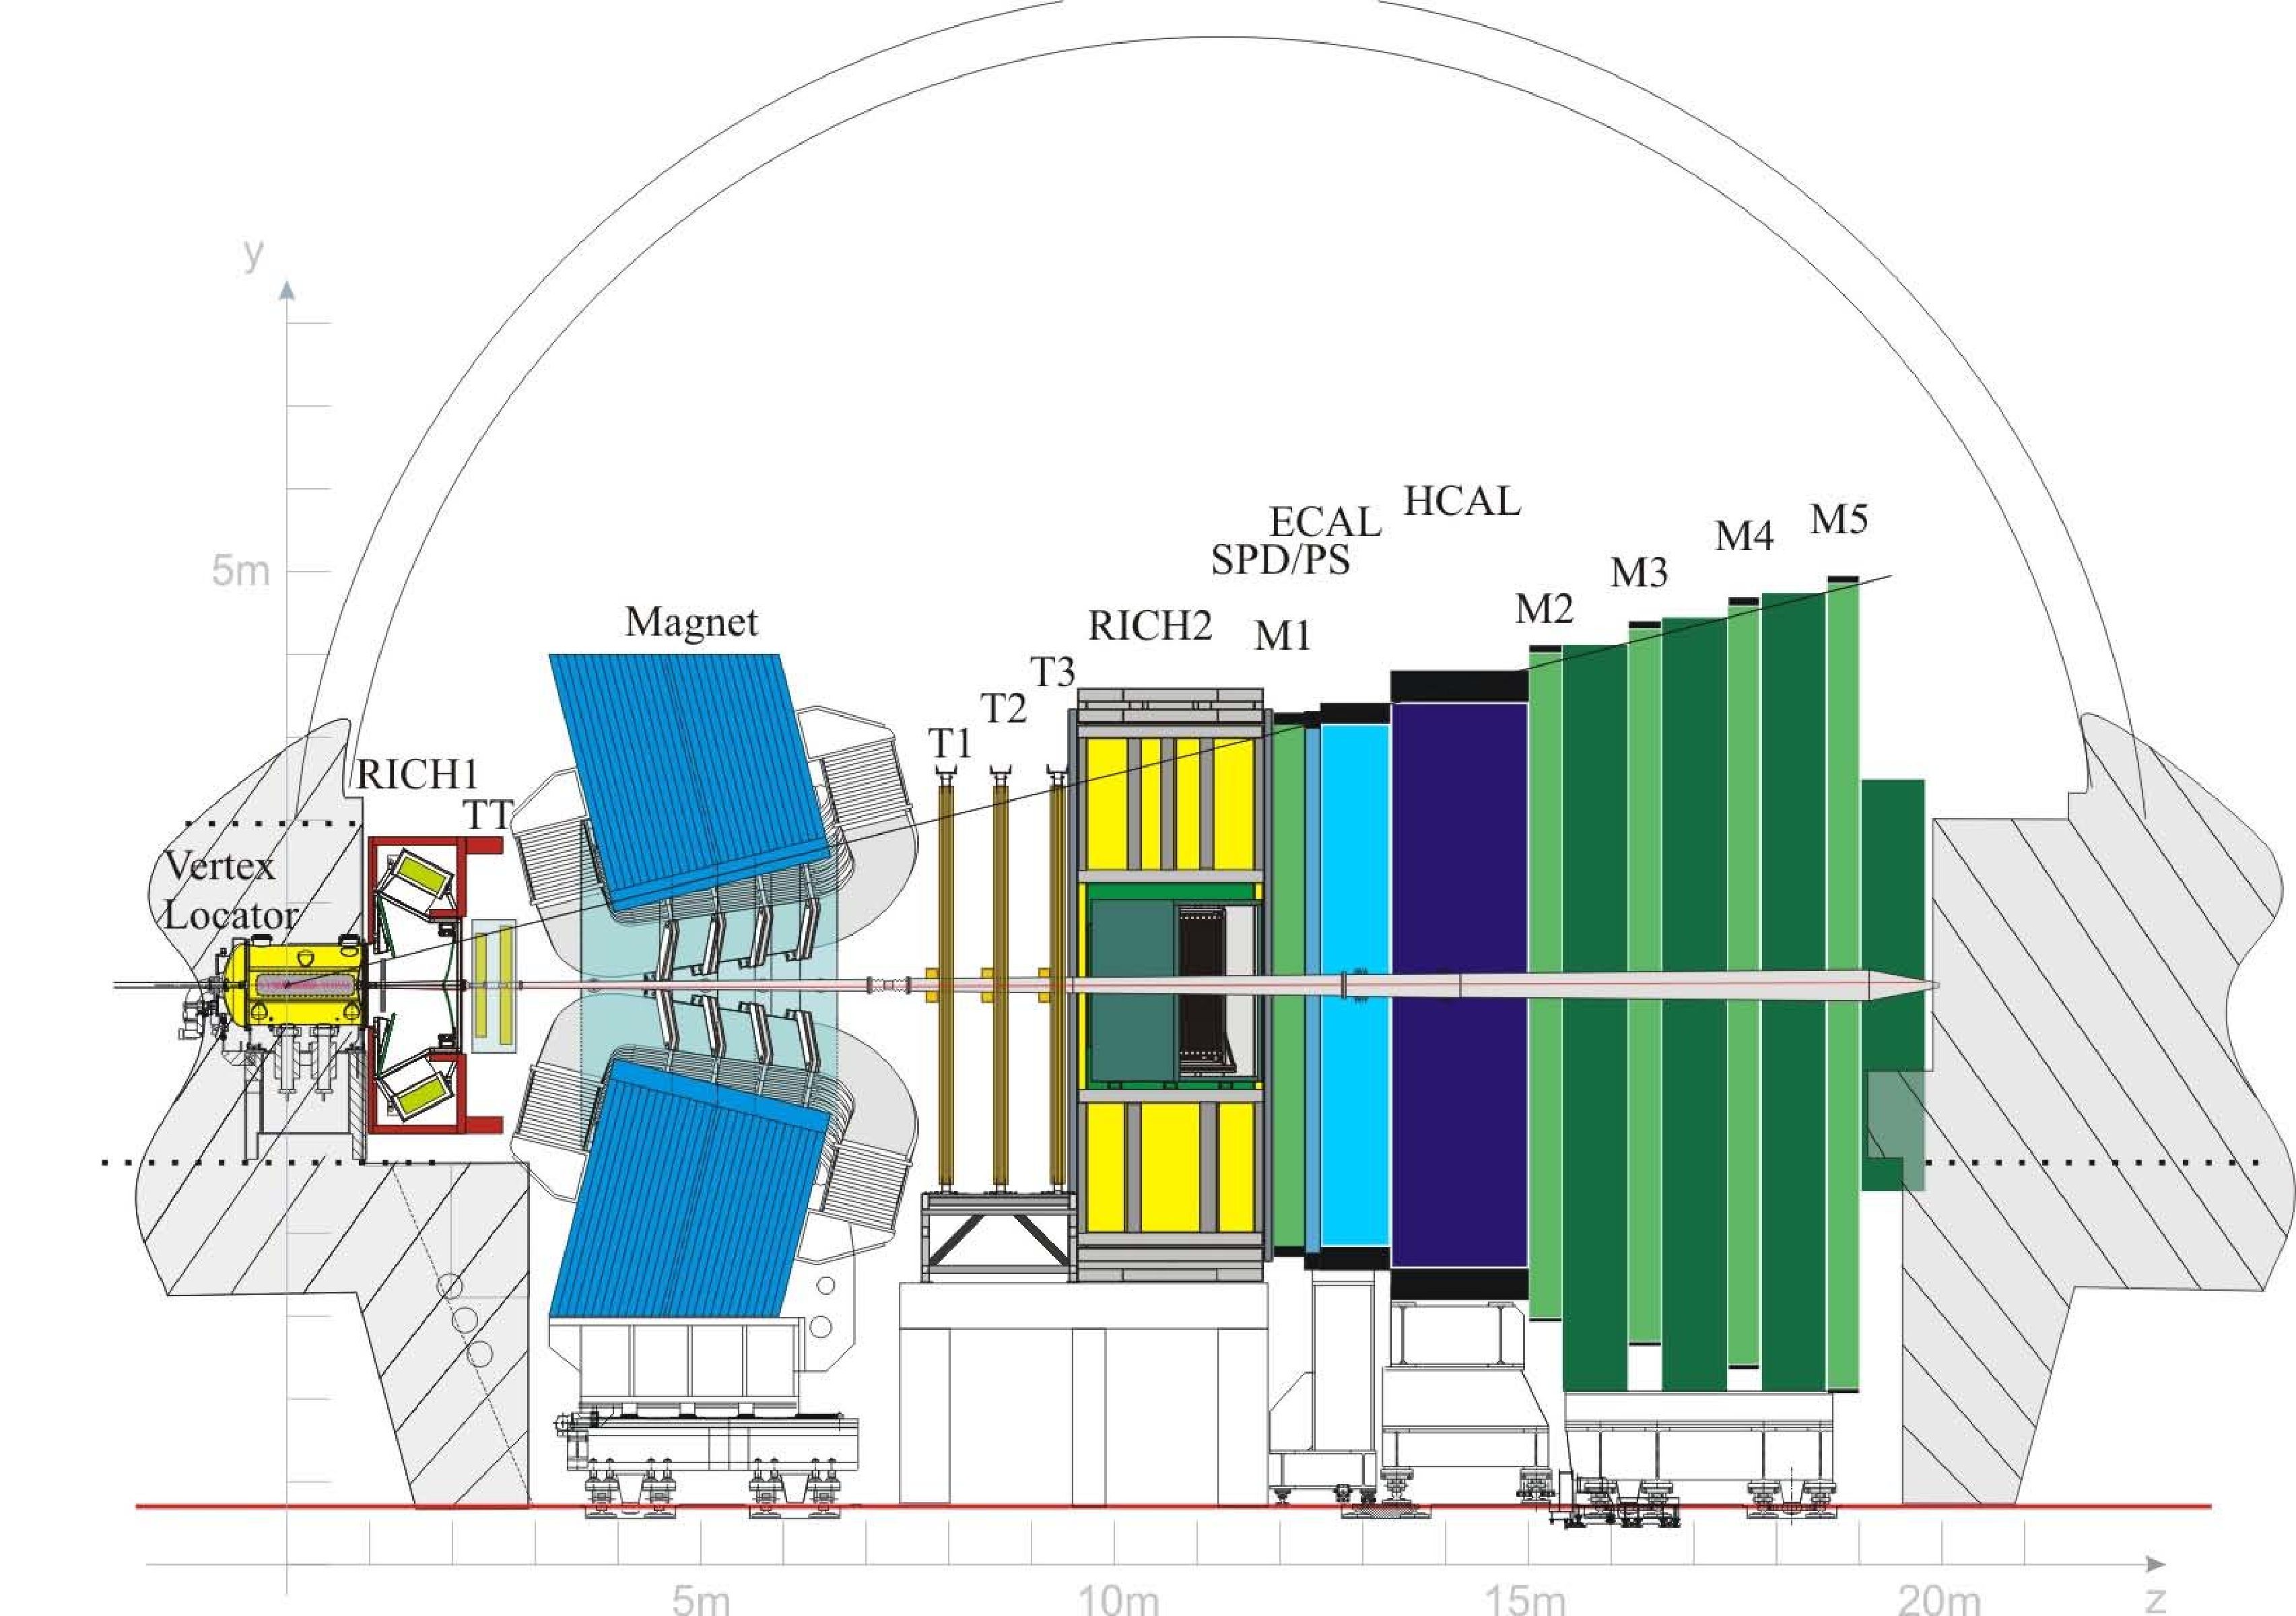
\includegraphics[scale = 0.15]{figs/detector/lhcbdet.pdf}
	\caption{The schematic slice of LHCb detector in $y,z$ plane where $z$ is defined to be the direction parallel to beamline, and $x,y$ define the plane perpendicular to the beamline. $\theta$, the opening angle in y-z plane with $\theta$ = 0 along $z-axis$.}
	\label{fig:LHCbDetector}
\end{figure}



\begin{table}[!h]
	\centering
	\hspace*{-0.8cm}
	\begin{tabular}{l c c c c }
		\hline
		 & $\sqrt(s)$ [TeV] & Luminosity $\mathcal{L}$ [$\times10^{32} cm^{-2}
		s^{-1}$] & Number of Bunches & Bunch Spacing [ns] \\ \hline
		2011 & 7  & 3.5 & 1300 &  50\\
		2012 & 8 & 4 & 1300 &  50\\
		2015 & 13 & 4 &  1.12 &  25\\      
		2016 & 13 & 4 &  1.12 &  25\\\hline      
		2017 & 13 & 4 &  1.12 &  25\\\hline      
	\end{tabular}
	\caption{}
	\label{tab:runcond}
\end{table}   

\begin{figure}
	\centering
	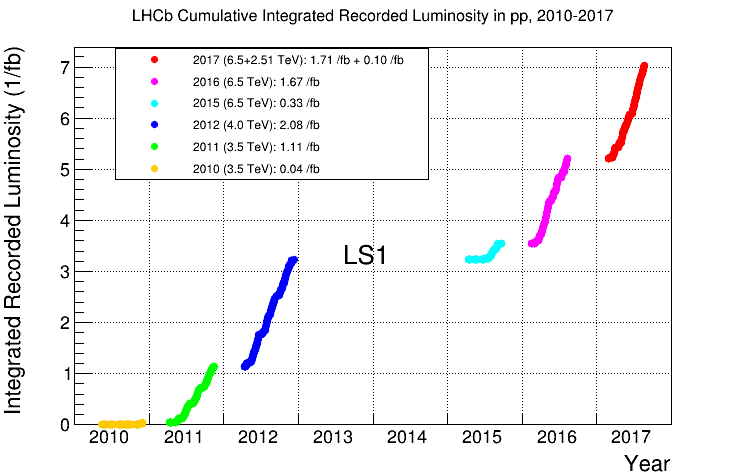
\includegraphics[scale = 0.5]{figs/detector/intlumi.png}
	\caption{Integrated luminosity collected in different years of data-taking. As compared to ATLAS and CMS the integrated luminosity is much lower, due to pile-up conditions. In 2017, there were two $pp$ collision energies at $\sqrt(s)$ =13 and 5 TeV.}
	\label{fig:lhcbintlumi}
\end{figure}


are hence heavily exploited at LHCb, with $pp\rightarrow b\bar{b}X$ This is compensated by preferential decays of containing $b$ particles in a specific angular region.  This region is defined along the beam pipe $\phi$ z-axis
